\documentclass[a4paper,12pt]{article}
\usepackage{mathtools,amsfonts,amssymb,amsmath,bm,commath,multicol}
\usepackage{algorithmicx, tkz-graph, algorithm, fancyhdr, pgfplots}
\usepackage{fancyvrb, amsthm, csquotes, booktabs, rotating}
\usepackage{appendix}
\usepackage[backend=biber, citestyle=authoryear]{biblatex}
\renewcommand*{\nameyeardelim}{\addcomma\space}
\addbibresource{thesis.bib}
\usepackage[noend]{algpseudocode}

\pagestyle{fancy}
\fancyhf{}
\rhead{Nandan Rao}
\lhead{Applying for jobs. When do you give up? }
\rfoot{\thepage}

\begin{document}

\title{ Applying for jobs. When do you give up?  }

\author{Nandan Rao}

\maketitle

\begin{abstract}

In the labor market, a clear implication of internet-based job applications is the ability for every worker to apply to more jobs without a corresponding increase in the firms' ability to interview more workers. In this paper I consider the interaction between this increased congestion and the search behavior of workers.

I hypothesize, and show preliminary experimental evidence that, statistical biases related to numerocity affect probabilistic judgement in such a way as to cause misjudgements in this context: faster ``applying'' is shown to potentially lead to earlier ``quitting.'' The suboptimality of this behavior is also proved.

I use estimations from the experimental evidence to calibrate a lightly extended version of the equilibrium directed search model of \cite{gonzalez2010}. Simulations show that this bias causes a hollowing-out of the middle class from the wage distribution, as high-skill workers who experience rejection direct their search to jobs with lower-than-optimal wages.

\end{abstract}



% This implies that a seemingly harmless technological improvement can have potential negative outcomes on the entire wage distribution due to the misjudgements of individual job seekers.

\section{Introduction}

Imagine a job seeker. They spend their first week looking and applying to jobs, and they submit their aplication to three different positions, all of which fit the profile of their ``dream job''. The next week comes around and they have not heard back from any of the firms. Should they continue to apply to the same type of job, or should they try to look for a job which might be easier to get?

Now consider an alternate universe, where the same job seekers spends their first week looking and applying to jobs, but now the time it takes to find and apply to each job has gone down, and they submit their application to 15 different positions, all of which still fit the profile of ``dream job''. The next week comes around, and they have not heard back from any of the firms. Should they continue to the same type of job?

This paper considers the way in which job seekers react to the above scenario: a technology change that reduces the cost of applying to jobs.

Recent history is rife with technologies that lower the cost of job search, from the fax machine to the internet to the integrated profile-cum-job-boards such as LinkedIn. It is not hard to imagine that yet more such technological changes await us in the near future. Given a reduction of costs, be they time or money, the number of applications sent per job seeker will, ceteris parabis, increase. As interviewing is still relatively unmediated by ``time-saving'' technologies, it is clear that the number of outright rejections the average job-seeker receives must naturally increase along with an increase in the number of applications the average job-seeker sends.

It is worth noting the difference between a technology lowering search costs and a technology lowering application costs. The cost of applying for a job consists of two parts: the cost of searching and the cost of actually sending the application. If one lowers the cost of searching, one would expect better-targeted applications. Lowering the cost of sending each marginal application, however, regardless of which part of the process changes, has an additional effect which is independent of the targeting: more applications are sent. I will not consider the effect of better-targeting applications in this paper, focusing instead on the potential effects of the increase in application volume independently of any other effects.

One might argue that probability of acceptance is actually the probability of winning a game which one is playing against all other potential applicants and all potential firms. In this paper I will assume that, in the game-theoretic taxonomy, this is an evolutionary game: there are too many other players to seriously claim that agents rationalize their strategies. Instead, they follow myopic strategies, and these myopic strategies inherently involve the estimatiion of the probability of getting each job before bothering to send the application.

How should we consider, then, the process of a job-seeker estimating the probability of getting a job, should they apply? Let us split the process into two parts:

1. The job seeker gathers, throughout their entire life, from family, friends, and school, a whole host of preconceptions about the state of the world and their own employability. They listen to the news, they hear rumors, they observe the experiencce of peers.

2. The job seeker applies to some jobs, and through the process of applying, learns more about the probability of recieving offers from each kind of job and firm to which they apply.

This paper considers only the second part, abtracting away from whatever priors the job seeker has from before, I consider how they update their beliefs through the process of applying.

The hypothesis of this paper is nothing more than ``if you get a lot of rejections when applying for a certain type of job, your think your chances of getting such a job are low.'' In and of itself, this is not very controversial and, Ceteris Paribus, this is exactly what any model of rationality would predict. The hypothesis here, however, is that even Ceteris very-much-not-Paribus, and even when one's chances of geting a job are not actually lower, job seekers in the real world might percieve them to be this way and act accordingly, even if it is not in their best interest, when presented with a large number of rejections.

The paper will proceed as follows: in section 2, I will introduce several theories from decision-theory that could potentially be at-play in this scenario. In sections 3 and 4, I introduce two laboratory experiments to test the way people react to the scenario, prove the optimal reaction, and analyze the results from participants recruited via Amazon's Mechanical Turk. In section 5, I describe an equilibrium model, a slightly extended version of the directed-search model of \cite{gonzalez2010}, and simulate results with parameters calibrated from the laboratory experiments. Finally, in section 6: conclusions and suggestions for further research.


\section { Judging Probabilities }

Does the way in which we, as humans, perform probabilistic calculations change as the numerocity of the problem increases? Several past results indicate yes:

\subsection{Ratio Bias}

A short family tree: Availability Hueristic (\cite{tversky1973}) begets Norm Theory (\cite{kahneman1986}) begets the Ratio Bias (\cite{miller1989}). Whereas the availability hueristic relates to memory, the ratio bias is purely about reported statistics, given in the moment.

The idiomatic ratio bias experiment goes as follows: there is a kid who really likes chocolate chip cookies, and thinks (like everyone) that oatmeal cookies are inferior. The kid goes to the cookie jar where there is 1 (10) chocolate cookie, and 19 (190) oatmeal cookies and picks one, supposedly without looking (as is the rule in the house). He comes back with a chocolate-chip cookie. Do you think he cheated (and looked)? Respondents answer this question differently based on whether there are 20 cookies or 200 cookies, even though the ratios are the same. Specifically, if there is 1 chocolate chip cookie (out of 20), people think it's more likely that the kid cheated (\cite{miller1989}). Often referred to as \textit{denomenator neglect}, there is the sense that we focus on the ``norm'' of the numerator, the size of it, in which 1 is less than 10, and therefore the event seems less likely.

\subsection{Numerocity Hueristic}

The origins of this idea can be traced back to a 1941 experiment showing that a kernel of corn, if divided into four pieces, is a more motivating reward for chickens than a single, undivided kernel (\cite{wolfe1941}). Humans, it turns out, are not so different, and systematically confuse numerocity (number of units) for quantity (actual amount). \cite{pelham1994} develops a framework, referred to as the numerocity hueristic, in which this bias is shown to be especially present when individuals attempt to make judgements while under cognitive load, in which case they fall back to numerocity as a rule-of-thumb for determining quantity. This line of research has been explored extensively in the consumer-behavior literature, where preferences are easily shifted based on a changing of scales (cite cite cite).

Is it plausible that, while deciding on the next job application to send, job seekers use ``number of rejections'' as a hueristic for ``expected value of sending one more application'', not fully taking into consideration the denomenator (time spent on each application) while doing so? I propose that this is exactly the case.

\subsection{Learning by Experience}

What about the way in which we judge the probability of rare events? It is worth noting that our context here is decidedly different from the one considered in prospect theory and its derivatives (\cite{kahneman1979}), which concern the judgement of probabilities based on external knowlege, primarily given via descriptions of the events. This distinction between \textit{decisions from description} and \textit{decisions from experience} is made in \cite{hertwig2004}, which gives a good overview of the field as well as decisive experiments which show the way in which decision-makers act differently, even oppositely, based on whether they learned about the probability of an event through trial-and-error or through written description.

Specifically, and opposed to Prospect theory, learning by experience is shown to cause people to \textit{underweight} the probability of rare events, both positive and negative. Note, that this seems very much to be independent of the Availability hueristic, which cites our ability to pull a representative example from memory (\cite{tversky1973}), as this result holds for experiments in which the participant has, immediately before, experienced both outcomes, and for ones in which they have not.

While this is in-and-of-itself interesting and applicable to this research, \cite{hertwig2004} notes one other curious fact that is not given an explanation: in the cited experiments, users are allows to ``sample'' from a given one-armed bandit as much as they like, a practise round without any specific end, before ``playing for keeps.'' Users, it seems, chronically undersampled: they quit practising sometimes before even coming accross the a rare outcome with a very large positive or negative reward, the knowledge of which would potentially change their behavior. 

This paper attempts to answer that very question: how do people estimate the probability of an unseen rare event? Do they ``snap'' their estimate to zero after not seeing the outcome in some number of chances, effectively assigning measure zero to events they have not seen?

\section{Experiment 1}

\subsection{ Experimental Design }

Participants are presented with an online web application, in which they click ``boxes''. These boxes can be thought of as slot machines. After they are clicked, they ``roll'' for a few moments (~1 second) and then present a result: either a green gem (signifying a ``win''), or a red skull (a ``loss''). If they find a green gem in any of the boxes they play, they are told the game will end and they will recieve a \$5 bonus.

Participants are randomly assigned to two groups. After some trial clicks, and being explained the rules, users are presented with a screen in which there are 3 (15) boxes. They ``play'' each box, and lose 3 (15) times. Next, they are presented with a screen asking them:

\begin{quote}
If you had the option to play another round (with another 3/15 boxes), what do you think the probability is that you will win a green gem in that round?
\end{quote}

After answering that question, participants are presented with the option to either take a \$2 participation bonus and quit the game, or forfeit the bonus and play one more round (where they have the chance to win \$5).

\subsection{ Proof of Optimality }

The problem is clearly a discrete 0,1 problem: either you find a green gem, or you do not (either you are rejected or you are accepted). The problem of learning then becomes one of estimating the free ($p$) parameter of a binomial distribution, given you have clicked $n$ boxes. Given your estimate, $\hat{p}$, the probability of winning at least one of the next $n$ attempts is given by:
\begin{equation} \label {eq:1}
  P(win) = 1 - (1-\hat{p})^n
\end{equation}
%
We will formulate the process of estimating $\hat{p}$ as one of Bayesian learning, with a Beta prior, paramaterized by $\alpha$ and $\beta$, on the value of $p$. Given $n$ failures, the corresponding posterior Beta distribution is paramaterized by:
\begin{align*}
  \alpha'_{n} &= \alpha \\
  \beta'_{n} &= \beta + n
\end{align*}
The PDF of the posterior estimate of $p$ after $n$ failed attempts is therefore given by:
$$
P(x | n) = \frac{ x^{\alpha - 1}(1 - x)^{\beta - 1 + n} \Gamma(\alpha + \beta + n)}{\Gamma(\alpha) \Gamma(\beta + n)} \implies x \sim \text{Beta}(\alpha, \beta + n)
$$
Which can be plugged back into \ref{eq:1} and take expectations to give us the expected payoff:
$$
\mathbb{E}[win] = \int_0^1 1 - \left( 1 - x \right)^n P(x | n) dx
$$
Which is increasing in $n$ for any valid values of $\alpha$ and $\beta$. Any reasonable estimate of $p$ compatible with correct Bayesian updating will, therefore, suggest that players estimate a greater probability of winning given another $n$ chances, after $n$ failures, as $n$ increases.

In other words, those presented with 15 failures, and given a chance for another 15 attempts, have a greater chance of winning than those with 3 failues and another 3 attempts.

\subsection{ Results }

The results from this experiment, while small in sample size (N = 30), are decidedly negative. This was a surprise to me personally, as previous versions of this same experiment with other incentives and different wording seemed to be yielding very large treatment effects in the reported estimated probability of winning the next round. Full results can be seen in table \ref{table:descriptive-1}.

While one should not draw definitive conclusions from such a small sample size, there might be something to the presentation of this problem that provides a countereffect to the learning-by-experience bias of estimating rare, unseen events. I will refrain from speculating futher, but believe this requires further research to understand the exact effects at play.

\begin{table}
  \caption{Summary Statistics for Experiment 1}
  \label{table:descriptive-1}
  \begin{center}
    \begin{tabular}{lcc}
      \hline
      & n = 15 & n = 3  \\
      \hline
      \hline \\ [-1.8ex]
      Median reported probability of winning &  50.00 & 47.00  \\
      \# who played 2nd round                 &   9 &  9  \\
      N                                  &   15 &  15  \\
      \hline
    \end{tabular}
  \end{center}
\end{table}

\section{ Experiment 2 }

\subsection{ Experimental Design }

This experiment was designed specifically for MTurk, taking advantage of several specific features of the platform and those who use it:

\begin{enumerate}
\item A job creater can specify the characteristics of those who see and can perform their job. This allows us to target, for example, only professional Turkers with a similar level of experience.
\item Turkers with similar qualifications have access to the same pool of jobs at any given time, and therefore similar opportunity costs.
\item On a daily basis, Turkers must decide which jobs are worth doing and which are not. So much so, that there are review websites\footnote{\url{https://turkerview.com}} set up, specifically so that Turkers can review job-posters, and in which they report the calculated hourly wage of the job. As such Turkers have, embedded in their very cultural institutions, a very explicit concept of opportunity costs and hourly wages while performing tasks.
\end{enumerate}

Participants are shown boxes which, similar to in experiment 1, can be played much like a slot machine and will randomly ``pay out'' with unknown but fixed probability. The boxes are shown to the participants one-at-a-time and the game ends when the participant wins a box or quits, whichever comes first. Participants are told, however, that they were randomly assigned to one of two groups: in the first, the probability of winning is small, in the second, the probability of winning is zero.

The treatment effect is on the speed of the box roll. Treatment group A can theoretically play a new box about once every 3 seconds. Group B, on the other hand, can only play a new box about once every 12 seconds.

We throw out the participants who got lucky and won, as the question is ``how many losses do you experience before you quit trying?''

\subsection{ Proof of Optimality }

In this game, as in applying to jobs, players two unknown variables to estimate, both of which effect the probability of winning:

\begin{enumerate}
\item The ``group'' the player belongs to ($a_i, i \in \{L,H\}$).
\item The (unkown) probability of payout, $t$, given that they are in the group $a_H$.
\end{enumerate}
%
Rolls are modelled as Bernouli random variables:
\begin{align*}
k_{n+1} \thicksim Bernouli( p ) \\
p \coloneqq P(a_H | n)P(t | n)
\end{align*}
Clearly, the two variables are not uniquely identifiable without further assumptions. In general, the difference between updating one's beliefs about one's own characteristics versus updating one's beliefs about the ``tightness'' of the labor market is extremely significant. In the scope of this experiment, however, participants' ``personal'' characteristics are given externally, by the experimenter, and it is not in any ways personal, permanent, or connected to ego. For this reason, in both this proof and in the empirical bias estimates we infer from the results, we model the joint estimation problem as one of estimating $p$ with the posterior mean $\hat{P}_n$ after $n$ failures, regardless of how exactly it is done, which allows us to model behavior in this particular situation without making any additional assumptions.

Clearly, this is an optimal stopping time problem, with the conditions for stopping given when the opportunity cost of playing ``one more roll'' exceeds the expected payoff, given the current estimation of p. Taking advantage of the fact that there is only one positive value $W$ can take, and making the assumption (for mathematical simplification) that agents use the posterior mean as a point estimate rather than integrating over the entire posterior distribution, we can thus charactize the optimal stopping time by:
$$
\hat{P}_n u(W) = u(tc)
$$
Where $t$ is the time (seconds) it takes to play one more roll, and c is the opportunity cost (dollars / second) of the outside option. Using this, we can comparing the stopping time between two groups, a and b, where $t_a = \frac{1}{x}t_b$. We want to prove that, as a parallel to the previous experiment, ``quicker'' plays should not cause earlier stopping. For this, it is enough to show that:
$$
\hat{P}_{xn}u(W) \geq u \left( \frac{tc}{x} \right)
$$
A proof is provided in Appendix \ref{appendix:proof}, where it is shown that this holds for any level of risk-aversion in a CRRA utility function. This proves that, rationally, quicker rolls does not lead to quicker quitting in optimal play.

\subsection{ Results }

Summary statistics of the results provided in table \ref{table:descriptive-3}.

In light of the previous proof, a natural first statistic to examine is the total time played by each group. Group A could, in theory, play four times as quickly as group B. Given our previous proof, however, group A should play \textit{ at least as } long as group B. Here, we see the opposite: the median time played by group A was about 240 seconds, while for group B it was around 311 seconds.

While indicative, this is not what we actually want to test. What we actually want to test is whether or not there exists a difference in the way in which they calculate $\hat{P}_n$, and the way it differs from the correct Bayesian estimation. If we knew the opportunity cost of time, $c$, and the utility function, we could back out their estimate of the probability:
$$
\hat{P}_n = \frac{u(tc)}{u(W)}
$$

Thus, it might be instructional to assume a functional form for the utility function, estimate the opportunity cost of time, which should be equally distributed for both groups, and examine that cost. These estimates are provided in table \ref{table:descriptive-3}, where one can see the results of a Mann Whitney U test between the distribution of costs for both groups.

A couple of facts jump out:

\begin{enumerate}
\item The implied opportunity costs are very large: about \$75 per hour for group A and \$50 for group B, assuming the identity utility function (risk nuetrality).
\item The implied opportunity costs of the two groups seem likely to come from different distributions.
\end{enumerate}

It thus appears that our participants decrease their probability estimate of winning too quickly. This is in accordance with the literature regarding probability estimation of rare events from experience (\cite{hertwig2004}), in which participants underestimate the probability of rare events. Additionally, we can weakly infer from this evidence that the strength of this bias is positively correlated with the numerocity of the problem: if increase the scale of the problem by speeding it up, you worsen the bias.



\section{ An Equilibrium Model }

How can biases of probability judgement affect the labor force on an aggregate level? Specifically, if these biases affect the way a job seeker decides where to search, what affects can these have on unemployment and wage distributions across the labor market?

In order to model such effects, we will need a model with:
%
\begin{enumerate}
\item Agent(s) that direct their search towards specific ``submarkets'' of jobs with different wage characteristics.
\item Agent(s) that do not know the objective probabilities of getting a job in any particular submarket, and must estimate these probabilities through a process of learning by experience.
\item Agent(s) that can experience both rejection and success in searching for jobs, and update their beliefs accordingly.
\end{enumerate}
%
A natural fit is to consider directed search models from the field of search and matching labor market models. Refer to \cite{wright2017} for a survey of directed search models.

There are several models from the directed search literature that attempt to model the effects of multiple applications directly (\cite{albrecht2006}, \cite{galenianos2009}, \cite{wolthoff2017}). These papers primarily focus on characterising the game between firms and workers when workes can recieve multiple offers at once and might reject an offer, and firms recieve multiple offers and once and must pick one to which they send the offer. While applicable to the larger contextual question of this paper, the focus is very different. This paper focuses on the process of learning an unknown probability of receiving a job, not the process of deciding where to apply once that probability has been estimated. 

\cite{gonzalez2010} offers a unique directed-search equilibrium model that fulfills all of the above requirements, and is the only model that I know of that does. 

\subsection{ Model Specification }

Please refer to \cite{gonzalez2010} for full specification of the model. 

For our purposes, I focus here on the the updating of beliefs. In the baseline model, workers are heterogeneous and endowed with skill $a_i, i \in \{ H, L \}$, and the exogenous distribution over the skills is known to everybody. All workers start with homogenous beliefs about their skill (the expected value given the exogenous distribution). They perform a dynamic programming excersize to determine the submarket with the highest expected value, and apply. Workers are matched to a job with probability $ax$, where $x$ is simply the submarket, continuously valued. After each ``round,'' workers update their beliefs via Bayesian updating, leading to an equilibrium tree of all possible beliefs and submarkets that are ``active.'' From this equilibrium tree, we extract the values of employment and unemployment.

It is easily shown that given the above assumptions, the posterior updates are:
%
\begin{align*}
  \phi(\mu) &\equiv  a_H + a_L - a_Ha_L/\mu \\
  H(x, \mu) &\equiv a_H - (a_H - \mu)(1 - xa_L)/(1 - x\mu)
\end{align*}
%
Where $\phi$ represents an update after a succesful match, and $H$ represents an update after a rejection. The posterior probability after $n$ rejections, $\hat{P}_n$, is then quite naturally defined within this model as the functional composition of $n$ posterior updates, such that the belief after 2 rejections is given by: 
$$
\hat{P}_2 \equiv H(g(H(g(\mu_0), \mu_0)), H(g(\mu_0),\mu_o))
$$
Thus, the posterior update after $n$ rejections, taking $\mu_0$ as given, takes the following form:  
%
$$
\hat{P}(n): \mathbb{N} \rightarrow \mathbb{R}
$$
%
I extend the model to incorporate a very simple and flexible bias parameter: 
%
$$
\hat{P}^{mod}(n) \equiv \hat{P} (n(1 + \epsilon))
$$
This bias linearly increases the number of rejections, such that a job seeker will react after 1 rejection as though they had receieved $1 + \epsilon$ rejections.

While flexible, this bias parameter does not fit into the functional form of our posterior estimate as defined above, only being defined on the natural numbers and therefore not defined on $N(1 + \epsilon), \epsilon \in \mathbb{R}$. 

To solve this problem, I take a first-order approximation of $\hat{P}^{mod}_n$, using finite differences from the surrounding naturals to numerically approximate the first derivative, thus defining $\hat{P}^{mod}_n: \mathbb{R} \rightarrow \mathbb{R}$ in the model space.

\subsection{ Calibration }

I use the empirical results from the second experiment to estimate the bias parameter, $\epsilon$, the only parameter I will explicitly calibrate.

A priori, we do not know the opportunity cost of time of each of the workers, but we can use the assumptions that A) they come from the same distribution and B) the distribution is limited in how spread it we believe it is, we can estimate the opportunity cost for each participant as:
$$
c_i \sim \text{Normal}(\mu_c, \sigma_c)
$$
Where $\mu_c$ and $\sigma_c$ are population parameters learned hierarchically with a weakly informative (half-Cauchy) prior on the mean and fairly strong inverse-gamma prior on the variance that shrinks it towards zero, thus grouping our cost estimates together as per our assumption. We then estimate a bias parameter for each individual::
\begin{align*}
  \epsilon_i \sim \text{Normal}(\mu_{\epsilon}, \sigma_{\epsilon})
\end{align*}
Where ``group'' parameters $\mu_{\epsilon, g}$ and $\sigma_{\epsilon, g}$ are learned hierarchically for each treatment group, $g$. I use an uninformative half-Cauchy prior on the median and weaker inverse-gamma prior on the variance. Exact specifications of all the model are available in the online supplementary materials and code.

We model the CRRA risk-aversion parameter, $\rho$, as:
\begin{align*}
  \rho \sim \text{Gamma}(3, 1)
\end{align*}
A weak prior with a mode of about 2. It is indicative that this parameter stays exactly at its mode, showing that our specification is robust to any reasonable parameter of risk-aversion. 

Finally:
\begin{align*}
  p_{i,g} = \frac{1}{1 + N_i(1 + \epsilon_g)}
\end{align*}
Where $p_{i,g}$ indicates the posterior mean estimated probability of winning of individual $i$ from group $g$ after $N_i$ rolls. We then ensure the condition:
$$
\frac{p_{i,g}}{c_i} = \frac{t_i}{W}
$$
Where $t_i$ is the mean time between each roll measured for participant $i$. For tractability, I transform this into a squared exponentiated loss function with a large penalization term, $\delta$:
$$
\exp \left\{ \delta \left(\frac{\hat{P}_n}{c} - \frac{t}{W} \right)^2 \right\}
$$

The theoretical model, while close, does not align exactly with the empirical model I have chosen. This is driven by several simple, and common, assumptions in the theoretical model:
%
\begin{enumerate}
\item All applicants know the probability of a succesful job application conditional on their skill level.
\item Skill level is a binary discrete variable (``low'' or ``high''), and as such the estimated posterior mean of this variable is a non-linear function of the numbers of rejections (or successes).
\item The probability of getting a job in any given submarket is linear in skill (the probability is given, simply, by $xa$, where $x$ is the submarket and $a$ is the skill level).
\end{enumerate}

The nature of the last two assumptions is that job seekers update their beliefs quickly after the first couple of rejections, and given the discretization of the submarket space into a reasonably small number of submarkets, they quickly end up searching the lowest possible submarket after a few rejections. Because of this quirk of the model, we cannot appropriately add in the exact biases that we have estimated: any bias over 1 will cause the same behavior. Thus, we calibrate the model by normalizing the lower bias to 0. In other words:

\begin{equation} \label {eq:epsilon-model}
\epsilon^{mod}_{g} = \frac{\epsilon_g - \min(\epsilon_g, \epsilon_{g'})}{\min (\epsilon_g, \epsilon_{g'})}
\end{equation}

Where $\epsilon_{g}$ is the empiricallly estimated bias for treatment group $g$, and $g'$ represents the other treatment.

\subsection{ Results }

Figure \ref{fig:posterior-mean-bias} shows the posterior distribution, calculated via Hamiltonian MCMC, of the two location parameters, $\mu_{\epsilon, g}$, which relate to the estimated mean bias within each treatment group.

It is worth noting that, sampling from this posterior, one can only reject the null hypothesis that the mean bias of group B is greater than or equal to group A at an 11\% level. This confidence level is in line with the inferences made directly from the simplistic opportunity costs calculated previously.

Full model parameters are provided in table \ref{table:model-params}, although these parameters should be considered extremely preliminary, as they were not calibrated specifically for this model. The results of posterior-updating bias on the wage-distribution outcomes, however, seem very robust to the rest of the model's calibration.

Figure \ref{fig:wage-distributions} shows the simulated wage distributions generated by the calibrated equlibrium model with bias parameter calculated as per (\ref{eq:epsilon-model}) using the median posterior values of $\epsilon_g$ as point estimates. While this is a stylized model, the results are nonetheless telling: greater bias leads to an erosian of the middle class. This is driven by high-skill workers who get unlucky in their first job application round: without the bias, they stay accurately hopeful about their own skill, and thus find a middle-wage job. With the bias, however, they become more pessimistic after a bit of bad luck, and immediately apply for (and get stuck in) lower-wage jobs.

\section{ Conclusions and Future Research }

Understanding how individuals direct their job search is crucial if we want to model the labor market and the impact of poilicies on its efficiency. I have argued that job search is, at its core, a process in which individuals must necessarily make judgements about the probabilities of favorable outcomes to different actions.

Learning by experience is one way in which invidividuals estimate these probabilities and this paper has focused on enumerating and testing some statistical biases related to learning by experience. In the experiments, and in the cited literature, I have only considered these biases in "impersonal" contexts. If one judges the probability of winning a "game" to be low, this has nothing to do with their own value or self-worth as an individual. If one judges the probability of getting a job to be low, this a lot to do with their own value and self-worth as individuals!

A simple extension and logical next step would therefore be to understand how learning-by-experience biases change when one is estimating something that might reflect positively or negatively on one's own self image. In the words of Anthony Greenwald (1980):

\begin{displayquote}
One of the best established findings in social psychology is that people perceive themselves readily as the origin of good effects and reluctantly as the origin of ill effects...
\end{displayquote}

It must also be considered that learning by experience is not the only, and may not even be the primary, way in which individuals estimate the probability of getting a job. Clearly, people do not apply to every single job they would enjoy doing: they know aprior that they are "not qualified" to do certain jobs, akin to estimating the probability of success to essentially zero in those contexts. This estimation involves preconceptions about the world that arguably might affect the way in which people direct their search much more than learning by experience, but also might very much affect the way in which people learn by experience. (cite) something about failures of bayesian updating in very generic way -- it's not only the prior that changes, but potentially also the updating itself.

This opens the question: how does public and private discourse effect the way in which people search for jobs? It is not hard to imagine that repeated exposure to negative discussions about the state of the economy and a high unemployment rate might come quickly to one's mind after a few rejections, even if it one felt quite confident beforehand.

Aditionally, I believe it is important to note that all of these affects might not only effect the directed search itself, but also the entire perception of bargaining power held by a majority of workers. If one underestimates the probability of getting a job, is one less likely to bargain for a higher wage, form a union, or petition for a raise after having worked for a while? In short, is it possible that a major change in the percieved bargaining power of workers can be caused by something as simple as a theoretically benevolent technological change that has the unfortunate side effect of increasing the absolute number of rejections for the majority of job seekers.




\printbibliography

\newpage

\begin{appendices}

\section{Tables \& Figures}
\label{appendix:graphs}


\begin{sidewaystable}
  \caption{Summary Statistics for Experiment 2}
  \label{table:descriptive-3}
  \begin{center}
    \begin{tabular}{lccccccc}
      \hline
      & Group & t &  Rolls  &  Time played & c ($\rho = 2$) & c (identity) & N \\
      \hline
      \hline \\ [-1.8ex]
      Median &         a &       4.00 & 54.00 & 239.91 &              0.25 &                      0.02 & 29  \\
      &         b &      15.00 & 18.00 & 311.39 &              0.07 &                      0.01 & 28  \\
      Mean   &         a &       4.52 & 76.72 & 374.41 &              0.27 &                      0.04 & 29  \\
      &         b &      16.89 & 23.71 & 400.08 &              0.07 &                      0.02 & 28 \\
      \hline \\ [-1.8ex]
      MW p-val & & & & 0.285 & 0.000 & 0.080 \\
      \hline \\ [-1.8ex]
      \multicolumn{6}{l}{\textit{Where $t$ is roll time and $c$ is opportunity cost in cents per second}} \\
    \end{tabular}
  \end{center}
\end{sidewaystable}

\begin{table}
  \caption{Model Parameters}
  \label{table:model-params}
  \begin{center}
    \begin{tabular}{lcc}
      \hline
      & Group B & Group A  \\
      \hline
      \hline
      B         &    0.70 &    0.70  \\
      aH        &    1.00 &    1.00  \\
      aL        &    0.05 &    0.05  \\
      b         &    0.03 &    0.03  \\
      bias      &    0.00 &    0.55  \\
      c         &    0.05 &    0.05  \\
      delta     &    0.01 &    0.01  \\
      precision &    0.01 &    0.01  \\
      r         &    0.04 &    0.04  \\
      sigma     &    0.10 &    0.10  \\
      y         &    0.11 &    0.11  \\
      \hline
    \end{tabular}
  \end{center}
\end{table}

\begin{figure}[h]
    \centering
    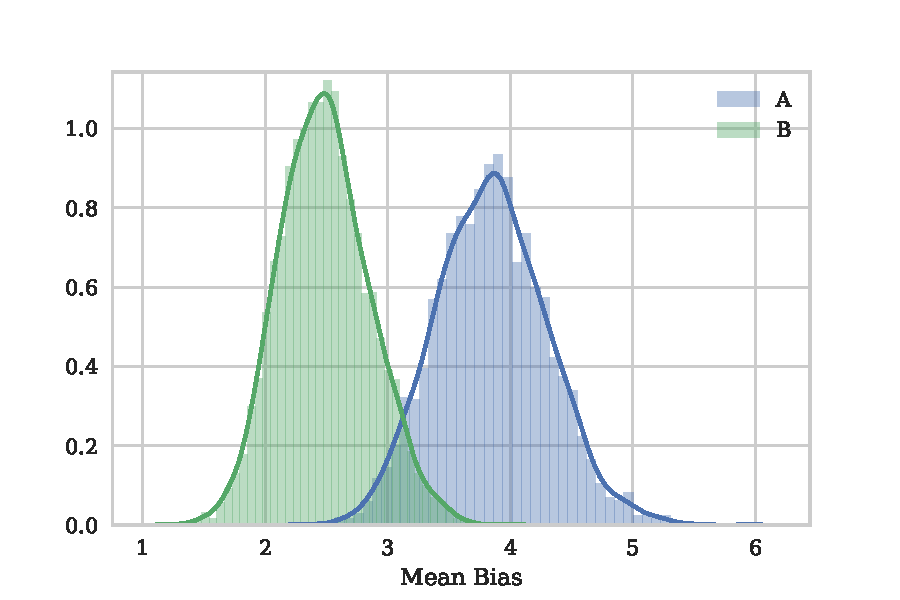
\includegraphics[width=0.95\textwidth]{../experiments/mean-bias}
    \caption{Posterior distribution for mean bias parameter}
    \label{fig:posterior-mean-bias}
\end{figure}

\begin{figure}[h]
    \centering
    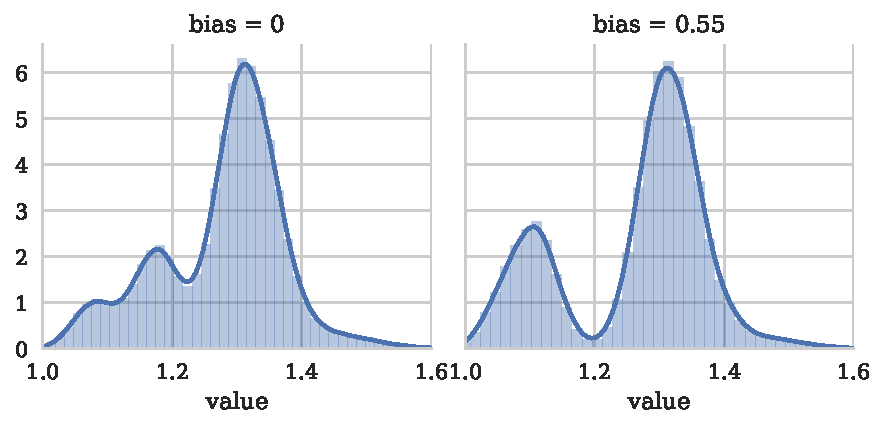
\includegraphics[width=0.95\textwidth]{../equilibrium/wage-distributions}
    \caption{Equilibrium wage distributions with estimated bias differential}
    \label{fig:wage-distributions}
\end{figure}

\newpage

\section{Proof of Non-Time Decreasing Optimality for Experiment 2}
\label{appendix:proof}

Given CRRA utility function:
\begin{align*}
u(c) =
  \begin{cases}
    log(c) \ \text{for} \rho = 1 \\
    \frac{c^{1 - \rho} - 1}{1 - \rho} \ \text{otherwise}
  \end{cases}
\end{align*}
%
We will prove separately, for both cases, that given:
\begin{align*}
  \hat{P}_{n}u(W) = u(tc)
\end{align*}
It follows:
\begin{equation} \label{proof:ineq}
  \hat{P}_{xn}u(W) \geq u(\frac{tc}{x})
\end{equation}
%
\paragraph{Log case}

Without loss of generality we assume the time per play is equal to one ($t = 1$) and solve for the revealed opportunity cost of time, $c$:
%
\begin{align*}
  \hat{P}_{n} \log(W) &= \log(c) \\
  c &= W^{\hat{P}_n}
\end{align*}
%
Which we plug into \ref{proof:ineq}
\begin{align*}
  \hat{P}_{xn} \log(W) &\geq \hat{p}_n \log(W) - \log(x)
\end{align*}
We use the fact that with reasonably large $n$, such that the data is large relative to the strength of the prior, the posterior mean is estimated by:
\begin{align*}
  \hat{P}_n \approx \frac{1}{n}
\end{align*}
Which we use to further develop our previous equation:
\begin{align*}
  \frac{1}{xn} \log(W) &\geq \frac{1}{n} \log(W) - \log(x) \\
 \log \left( W^{\frac{1}{xn}} \right) &\geq \log \left( \frac{W^{\frac{1}{n}}}{x} \right) \\
  x W^{\frac{1}{xn}} &\geq W^{\frac{1}{n}}
\end{align*}
Which holds, again, for any reasonably large $n$ such that $W^{\frac{1}{n}} \rightarrow 1$ and $x > 1$. Numerical proofs are provided in the online suppliments showing that these assumptions of large $n$ are a mathematical convenience and that the result holds for all feasible values of $n \geq 1$ and $x > 1$.

\paragraph{General case}

Again, assuming without loss of generality that $t = 1$ we solve for the opportunity cost of time. Note, I drop the minus one in the numerator, as is customary for convenience, which has implications discussed further down:
\begin{align*}
  \hat{P}_n u(W) &= u(c) \\
  \hat{P}_n  \frac{W^{1 - \rho}}{1 - \rho} &= \frac{c^{1 - \rho}}{1 - \rho} \\
  c &= \left( \hat{P}_n W^{1 - \rho} \right)^{\frac{1}{1 - \rho}} \\
  c &= \hat{P}_n^{\frac{1}{1 - \rho}} W
\end{align*}
%
Developing \ref{proof:ineq} with the revelead cost and imposing $\rho > 1$, we solve for the risk-averse case, the opposite being symmetric:
\begin{align*}
  \hat{P}_{xn}  W^{1 - \rho} &\leq \frac{c}{x}^{1 - \rho} \\
  x \hat{P}_{xn}^{\frac{1}{1 - \rho}}  W &\geq c \\
  x \hat{P}_{xn}^{\frac{1}{1 - \rho}}  &\geq \hat{P}_n^{\frac{1}{1 - \rho}}
\end{align*}
As in the log case, we impose relatively large $n$ to approximate the posterior:
\begin{align*}
  x \left( \frac{1}{xn} \right)^{\frac{1}{1 - \rho}}  &\geq \left( \frac{1}{n} \right)^{\frac{1}{1 - \rho}} \\
  x^{\frac{ - \rho}{1 - \rho}}  &\geq 1
\end{align*}
Which is clearly satisfied for all $\rho > 1$. Again, numerical proof is provided without the simplifying assumptions in the online suppliments.



\end{appendices}
\end{document}